%% This is an example first chapter.  You should put chapter/appendix that you
%% write into a separate file, and add a line \include{yourfilename} to
%% main.tex, where `yourfilename.tex' is the name of the chapter/appendix file.
%% You can process specific files by typing their names in at the 
%% \files=
%% prompt when you run the file main.tex through LaTeX.
%% prompt when you run the file main.tex through LaTeX.
\chapter{Evaluating the GEOS-Chem Predictions of Mercury Concentrations in the Atmosphere }
%% BACKGROUND
\section{Background}


\begin{flushleft}
Mercury (Hg) is found pervasive in the atmosphere and can accumulate in ecosystems, where it is transformed to its highly toxic form (methyl-Hg), which is destructive to ecosystems. Moreover, Hg lasts a long time in the atmosphere, allowing it to travel to faraway places resulting in  its elemental form, \hg \ being distributed globally through the atmosphere \cite{horowitz_new_2017,shah_improved_2021}.Approximately 90 to 99 percent of Hg is observed in the atmosphere as Gaseous Elemental Mercury (GEM/Hg0). Furthermore, both ocean and terrestrial surfaces emit elemental mercury (Hg0). In contrast, most deposited mercury (dry or wet) is oxidized mercury (HgII). Since most Hg entering ecosystems comes from the atmosphere, it is essential to monitor and model atmospheric Hg and Hg deposition to develop policies to curb the negative impacts of Hg on people and the environment.
\end{flushleft}
\begin{flushleft}

Modeling Hg's atmospheric chemistry transport using CTMs is crucial to understanding it's sources, processes, and fate. Furthermore, models such as GEOS-Chem allow us to understand the natural world and predict its future by approximating the behavior of various chemical species in the atmosphere. Consequently, identifying, quantifying, and minimizing model errors is essential, and observations of the atmosphere are crucial resources to do so. Evaluating a model with an ensemble of observations helps check consistency of a observations and enables constraints from multiple sources to be considered\cite{brasseur_modeling_2017}.
 \end{flushleft}
\begin{flushleft}
 
It is crucial to monitor ambient Hg data on a global scale over time in order to assess its emissions, transportation, atmospheric chemistry, and deposition. Brasseur and Jacob, (2017) prescribe that having a large ensemble of observations is vital for model evaluation. Therefore, it is of no surprise that evaluation of Hg models with observational data is an active area of research with a wide range of studies analyzing different characteristics of Hg in the atmosphere. These include emissions, atmospheric chemistry, removal processes, modeling, and historical trends. Moreover, region specific modelling studies are presented featuring the polar regions, Europe, North America and East Asia. However, no detailed modelling studies are presented for some of the regions that are reported to have high anthropogenic Hg emissions such as Latin America and Africa. Moreover, an extensive scan of numerous modelling studies to identify the extent to which regions such as Latin America, Africa and South East Asia are analyzed in the context of model observation comparison resulted in no studies being found. The dearth of studies that analyze these regions may be attributed to the fact that these regions historically and currently lack enough Hg long term monitoring capacity as depicted in Figure \ref{fig:global-hg-monitoring-networks} which shows the distribution of global Hg monitoring networks as published in the GMA 2018. 
\end{flushleft}

\begin{figure}[H]
  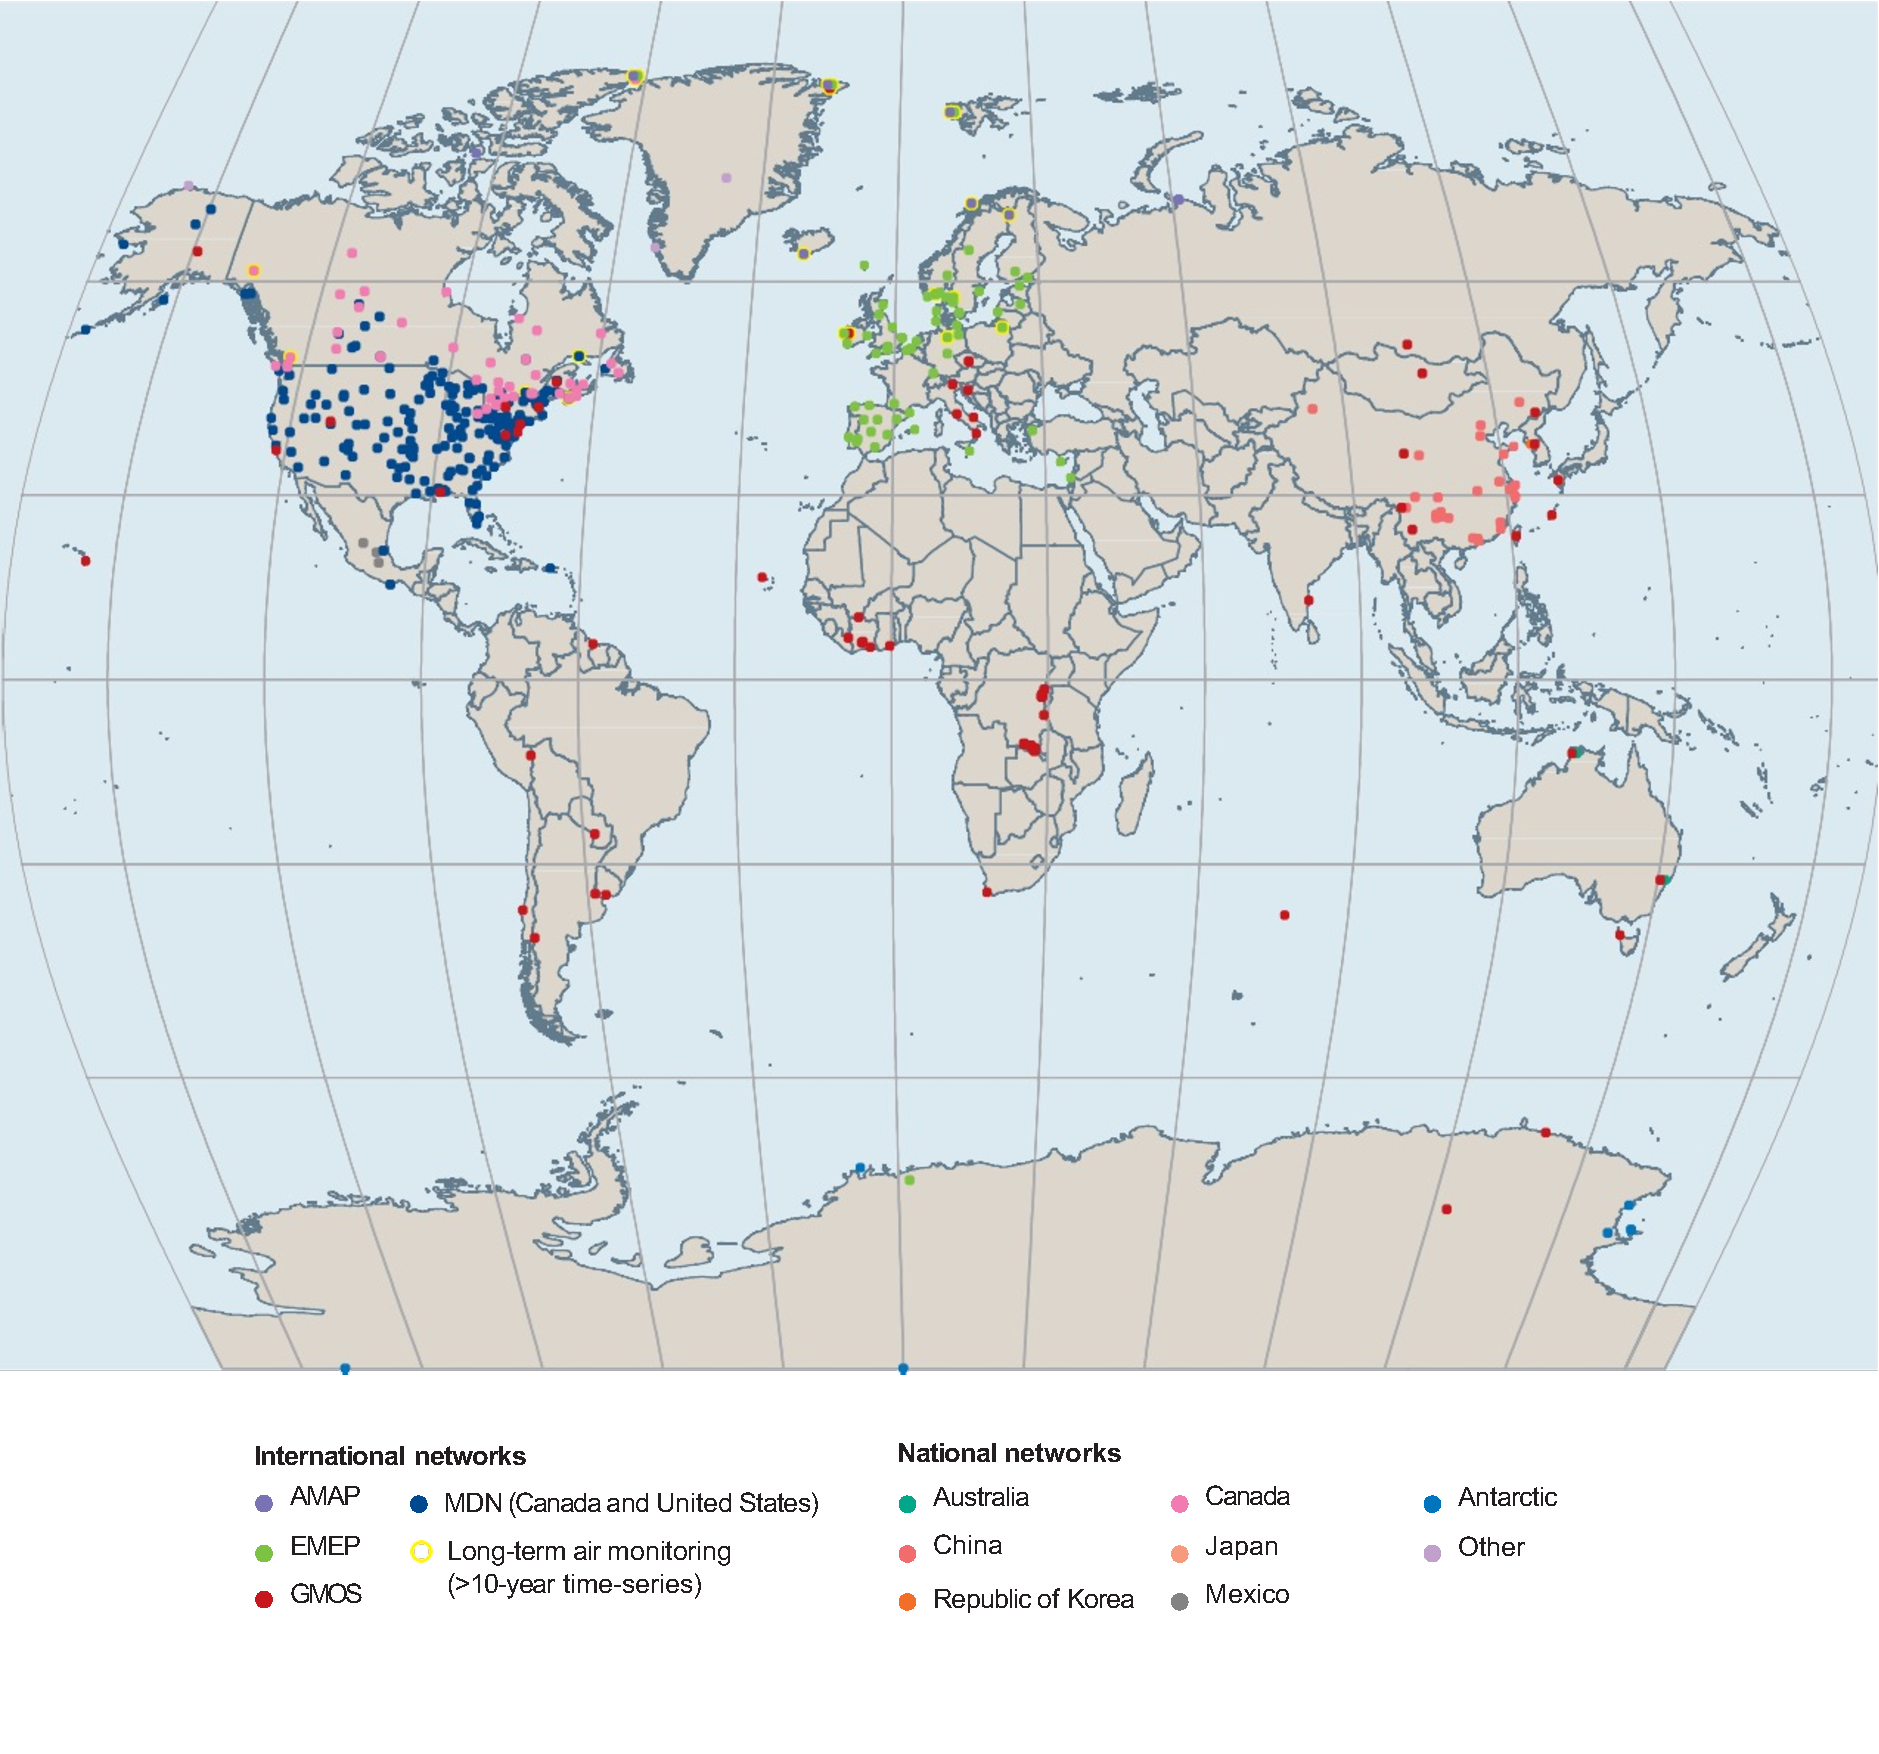
\includegraphics[width=\textwidth]{templates/figures/global-hg-monitoring-networks.pdf}
  \caption{Global map of Hg monitoring networks \cite{united_nations_environment_programme_technical_2019}}
  \label{fig:global-hg-monitoring-networks}
  \centering
  
\end{figure}
\FloatBarrier

\begin{flushleft}
 As seen on Figure \ref{fig:global-hg-monitoring-networks}, Latin America, Africa and South East Asia are significantly behind Europe, and North America regarding access to the relevant observation ensembles to track the evolution of Hg in the atmosphere. Regardless of the dearth of a large ensemble  of observations in Latin America, I present analysis and evaluation of atmospheric Hg concentrations simulated by the GEOS-Chem model with measurements recorded at multiple sites in Latin America including total gaseous mercury (TGM) measurements from the Global Mercury Observation System (GMOS) and gaseous elemental mercury (GEM) concentration data from a network of passive air samplers (PAS) distributed across Latin America.
\end{flushleft}




%%----------------------------METHODS-------------------------------------------
\section{Methods}
\subsection{GEOS-Chem}
\begin{flushleft}
% The GEOS-Chem model \cite{bey_global_2001} was used to simulate atmospheric concentrations of Hg for comparison with data constraints. GEOS-Chem is a global-scale, 3-D atmospheric chemical transport model driven by meteorological input from the Goddard Earth Observing System (GEOS) of the NASA Global Modeling and Assimilation Office. It runs at a resolution of 0.25° latitude x 0.3125° longitude horizontally, equivalent to $\approx$27 km at the equator, and 72 levels in the vertical. Numerous atmospheric chemical species have been simulated using GEOS-Chem, including Hg \cite{amos_gas-particle_2012,holmes_global_2010,selin_chemical_2007,selin_global_2008,zhang_naturally-derived_2016}. Travnikov et al. (2017) also used GEOS-Chem for international model comparisons to support the Global Mercury Assessment and the Minamata Convention on Mercury \cite{travnikov_multi-model_2017}.

The Hg concentration in the atmosphere was simulated using version 12.8.0 of GEOS-Chem at a resolution of 2.0$\times$2.5, which is approximately equal to a 222 km$\times$277.5 km grid square at the equator and 47 vertical layers\cite{horowitz_new_2017}.Moreover, the MERRA-2 assimilated meteorological data drive's the model's atmospheric transport \cite{gelaro_modern-era_2017}. The GEOS-Chem Hg model calculates Hg trasport in the atmosphere in three tracers: elemental Hg, Hg\textsuperscript{0}, divalent Hg, Hg\textsuperscript{2+}, and particulate-bound divalent Hg,Hg\textsuperscript{p}. Furthermore, the GMA 2018 emissions inventory was used to represent anthropogenic emissions sources from all sectors\cite{steenhuisen_development_2019}. Different inputs to the GEOS-Chem model such as emissions sources can be toggled on or off depending on the research objective, hence a reference simulation, \on was created by turning on all Hg emissions sources globally. Moreover, a \off was generated by turning off the ASGM source globally to evaluate the contribution of ASGM to the baseline \hg in the atmosphere by calculating difference between the \on and \off.
\end{flushleft}

\begin{table}[H]
\captionof{table}{Description of GEOS-Chem Simulations Conducted}
\label{tab:geos_chem_simulation_description}

\centering
\resizebox{\textwidth}{!}{\begin{tabular}{lcp{0.6\linewidth}}

Simulation Name  & Resolution & Description  \\
                        
\hline
Base (ASGM=ON)         & 2.0$\times$2.5 & All Hg anthropogenic emission sources are turned on  \\
No ASGM(ASGM=OFF)        & 2.0$\times$2.5 & All Hg anthropogenic emission sources are turned on except ASGM emissions 

\end{tabular}}

\end{table}

\begin{flushleft}

 The frequency of the simulation output set set to output daily \hg averages at the global scale while the \hg output for the grid boxes corresponding to the locations of the observation sites was set to a hourly frequency. The GEOS-Chem outputs for all the simulations conducted were in units of parts per trillion (ppt) and were converted to \nang at standard temperature and pressure (273 K, 1 atm) to compare them to observations.
\end{flushleft}

\subsection{Observation Data}

\begin{flushleft}
 The Global Mercury Observation System (GMOS) is one of a few major global projects aimed at developing a global observing system for mercury pollution. A vast network of ground-based monitoring stations, regular oceanographic cruises, and lower, upper, and stratospheric measurements make up this European-funded project \cite{sprovieri_atmospheric_2016} \cite{koenig_seasonal_2021}. More than 40 ground-based monitoring sites constitute the international network, covering many regions with limited to no observational data available before GMOS. The GMOS monitoring network sites in Latin America are shown by the dots with red outline on Figure \ref{fig:GMOS_PAS_stations_map}. Available Hg observation data from the GMOS stations on Figure  \ref{fig:GMOS_PAS_stations_map} was obtained from the GMOS online database as well as published studies about the Hg monitoring data from the different sites \cite{koenig_seasonal_2021}.  
\end{flushleft}
\begin{figure}[H]
  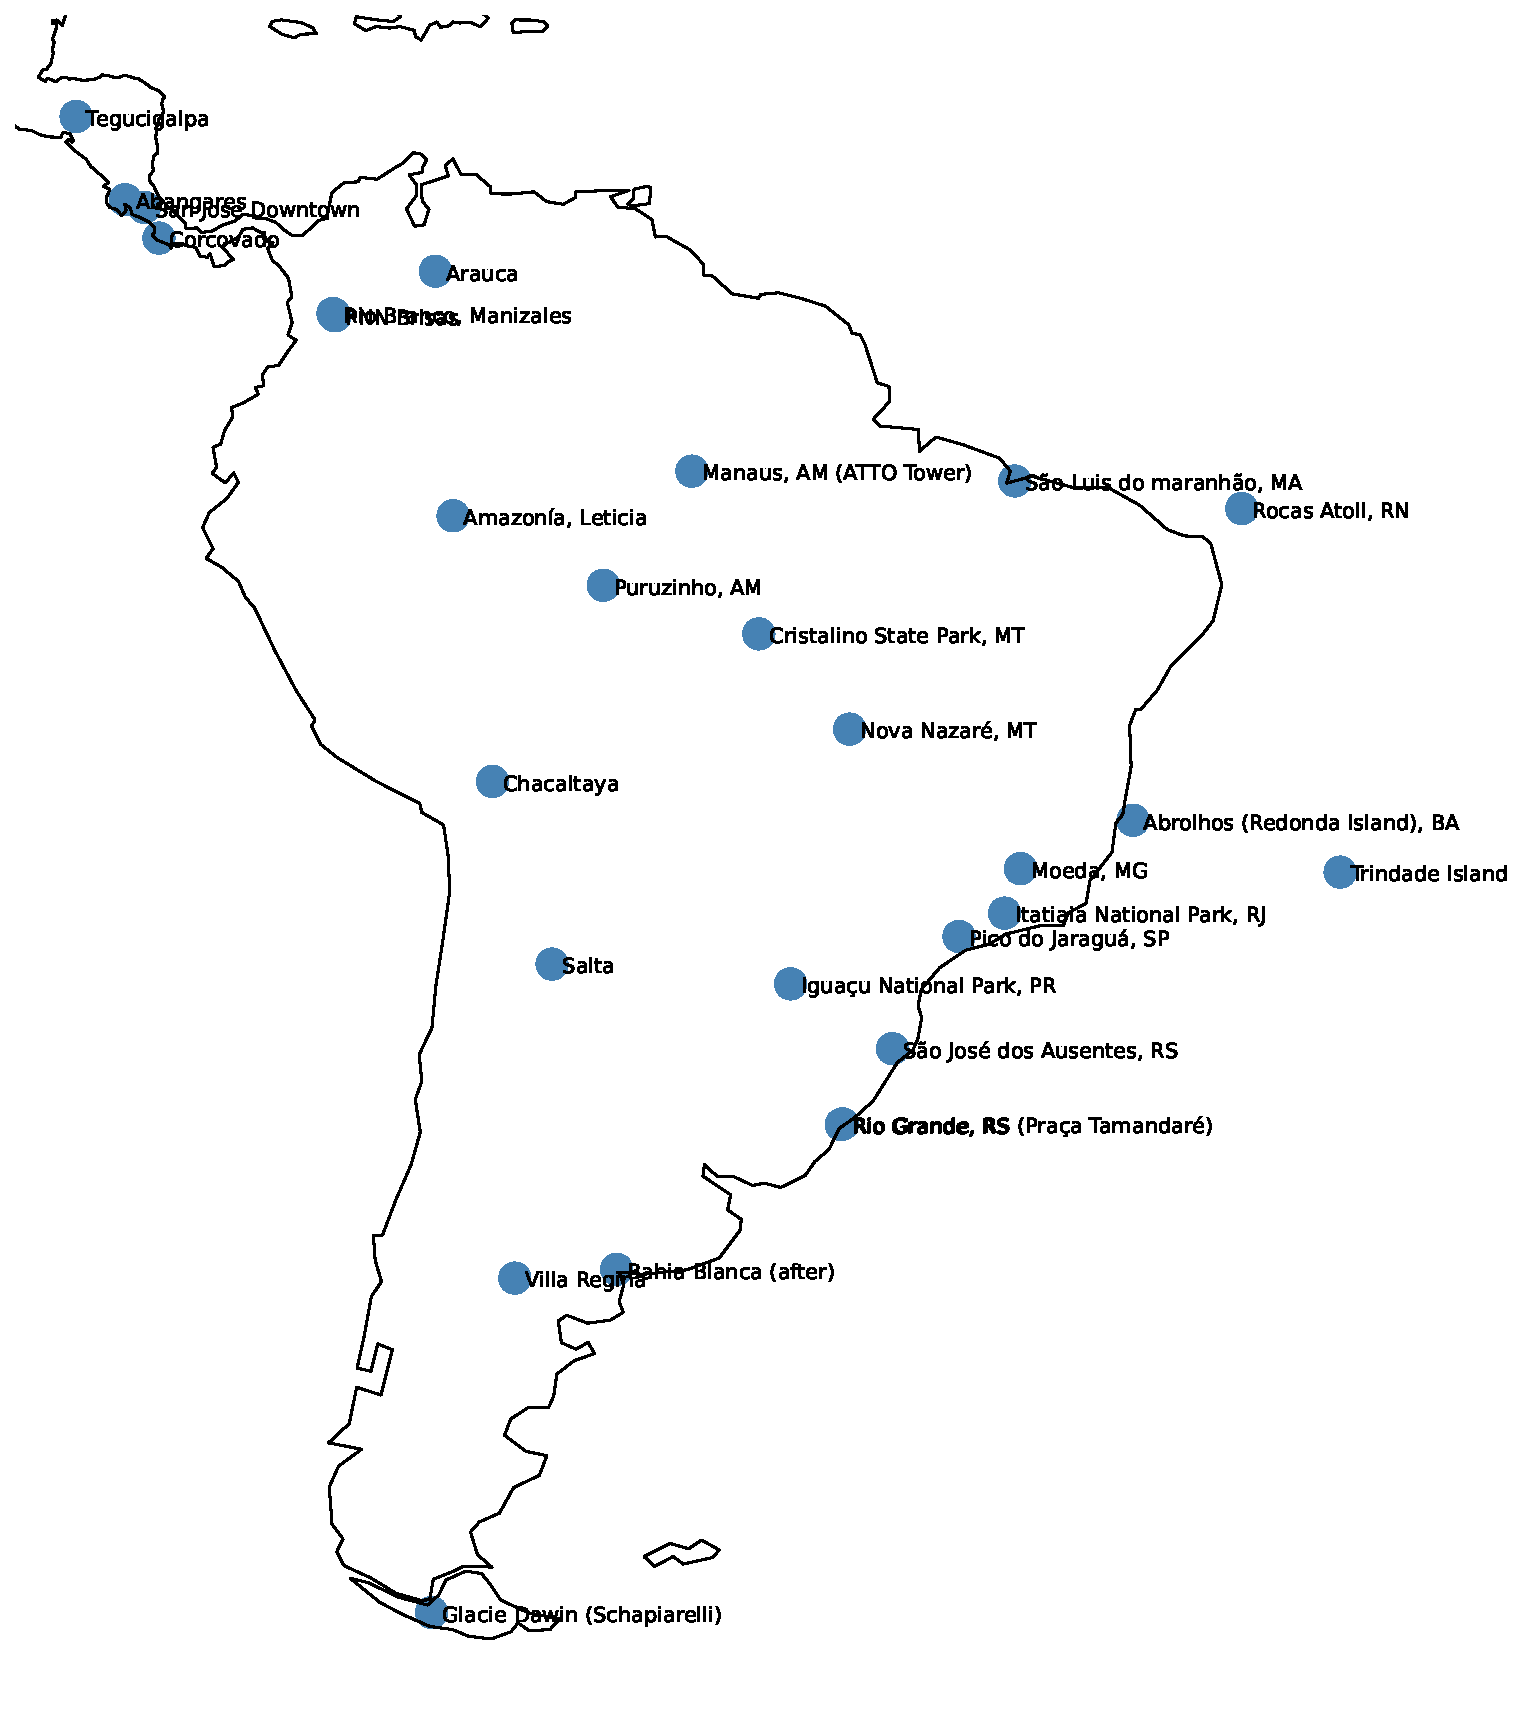
\includegraphics[width=0.8\textwidth]{templates/figures/Passive_Samplers/Latam_Passive_SamplerSites.pdf}
  \caption{Map Showing the GMOS Monitoring Network Sites and Passive Sampler Locations in South America}
  \label{fig:GMOS_PAS_stations_map}
  \centering
  
\end{figure}
\FloatBarrier

\begin{flushleft}
The hourly measurements of total gaseous mercury (TGM) in the atmosphere in \nang was retrieved, converted to daily averages and compared to the GEOS-Chem modelled \hg at the various sites for the period between 2012 and 2016. In contrast to Hg monitoring equipment such as those used in the GMOS network, which can be prohibitively expensive, energy-intensive, and require extensive training, passive air samplers (PAS) require no energy to operate and do not require any special handling skills. Furthermore, PAS can be easily deployed for long periods. This combination of attributes of PAS allows more sampling sites to be studied over a extended periods enabling significant average GEM concentration estimates to be obtained. Average annual GEM concentration data for 27 sites in Latin America as shown by the blue dots on Figure  \ref{fig:GMOS_PAS_stations_map}. The data set was obtained from Quant et al., (2021), which included information about the coordinates of the deployment sites and the period of measurement\cite{quant_measuring_2021}. The PAS data was compared to the annual average Hg concentration for the year 2015 and the coordinate information from the PAS data was used for direct comparison of the GEM observations and model outputs at the respective PAS sites.
\end{flushleft}


%%----------------------------RESULTS AND DISCUSSION---------------------------
\section{Results and Discussion}
\subsection{GMOS Observations vs GEOS-Chem}

\begin{flushleft}
A striking trend apparent in most of the plots of the observed vs modeled Hg concentration on Figure \ref{fig:GMOSvsGC} is the GEOS-Chem model's general overestimation of the Hg concentration and mismatch in the variability. The observed average daily TGM concentration at the GMOS sites (red line) is compared to the modeled \on average daily \hg (blue line) and the ASGM contribution (black line). The different Hg concentrations were plotted as a function of time based on the availability of data records between 2012 and 2016. None of the sites had a continuous data set that spanned the entire period of interest but the Niew Nickerie and Manaus sites had the least data records at 215 and 100 respectively as seen on Table \ref{tab:ASGM_at_GMOS_annual_avs}.   
\end{flushleft}
\begin{table}[H]
\captionof{table}{The comparison of the model predictions of the average Hg concentration for a 1 year measurement period}
\label{tab:ASGM_at_GMOS_annual_avs}

\centering
\resizebox{\textwidth}{!}{\begin{tabular}{lcccccc}
  \hline

GMOS  &Number of& Observed Hg\textsuperscript{0} & Observation Standard & Base(ASGM=ON) Hg\textsuperscript{0} & Base(ASGM=ON) Standard  & ASGM Contribution  Hg\textsuperscript{0}   \\
Site & Records & (ng m$^{-3}$)/year             & Deviation ($\sigma$) & (ng m$^{-3}$)/year                   & Deviation ($\sigma$)      &(ng m$^{-3}$)/year\\
                        
\hline
Sisal          & 320 &1.19 & 0.14 & 1.27 & 0.05 & 0.12  \\
Calhau         & 309 &1.22 & 0.12 & 1.30 & 0.04 & 0.11  \\
Niew Nickerie  & 215 &1.11 & 0.23 & 1.41 & 0.06 & 0.25    \\
Manaus        & 100 &1.49  & 0.31 & 1.27 & 0.09 & 0.23   \\
Chalcataya     &333 &0.90 & 0.16 & 1.20 & 0.14   &0.28   \\
  \hline
\end{tabular}}

\end{table}



\begin{flushleft}
Another significant aspect of the model observation comparison on Figure \ref{fig:GMOSvsGC} is the low predicted ASGM contribution at  four of the GMOS sites in contrast to the variability that closely matches the observed variability at the Chalcataya (CHC) site. A plausible explanation of models predicted ASGM contribution to the \hg at the GMOS location may be attributed to the CHC site's proximity to the Madre de Dios region in Peru which is a known source of enormous ASGM Hg emissions. 
\end{flushleft}

\begin{figure}[H]
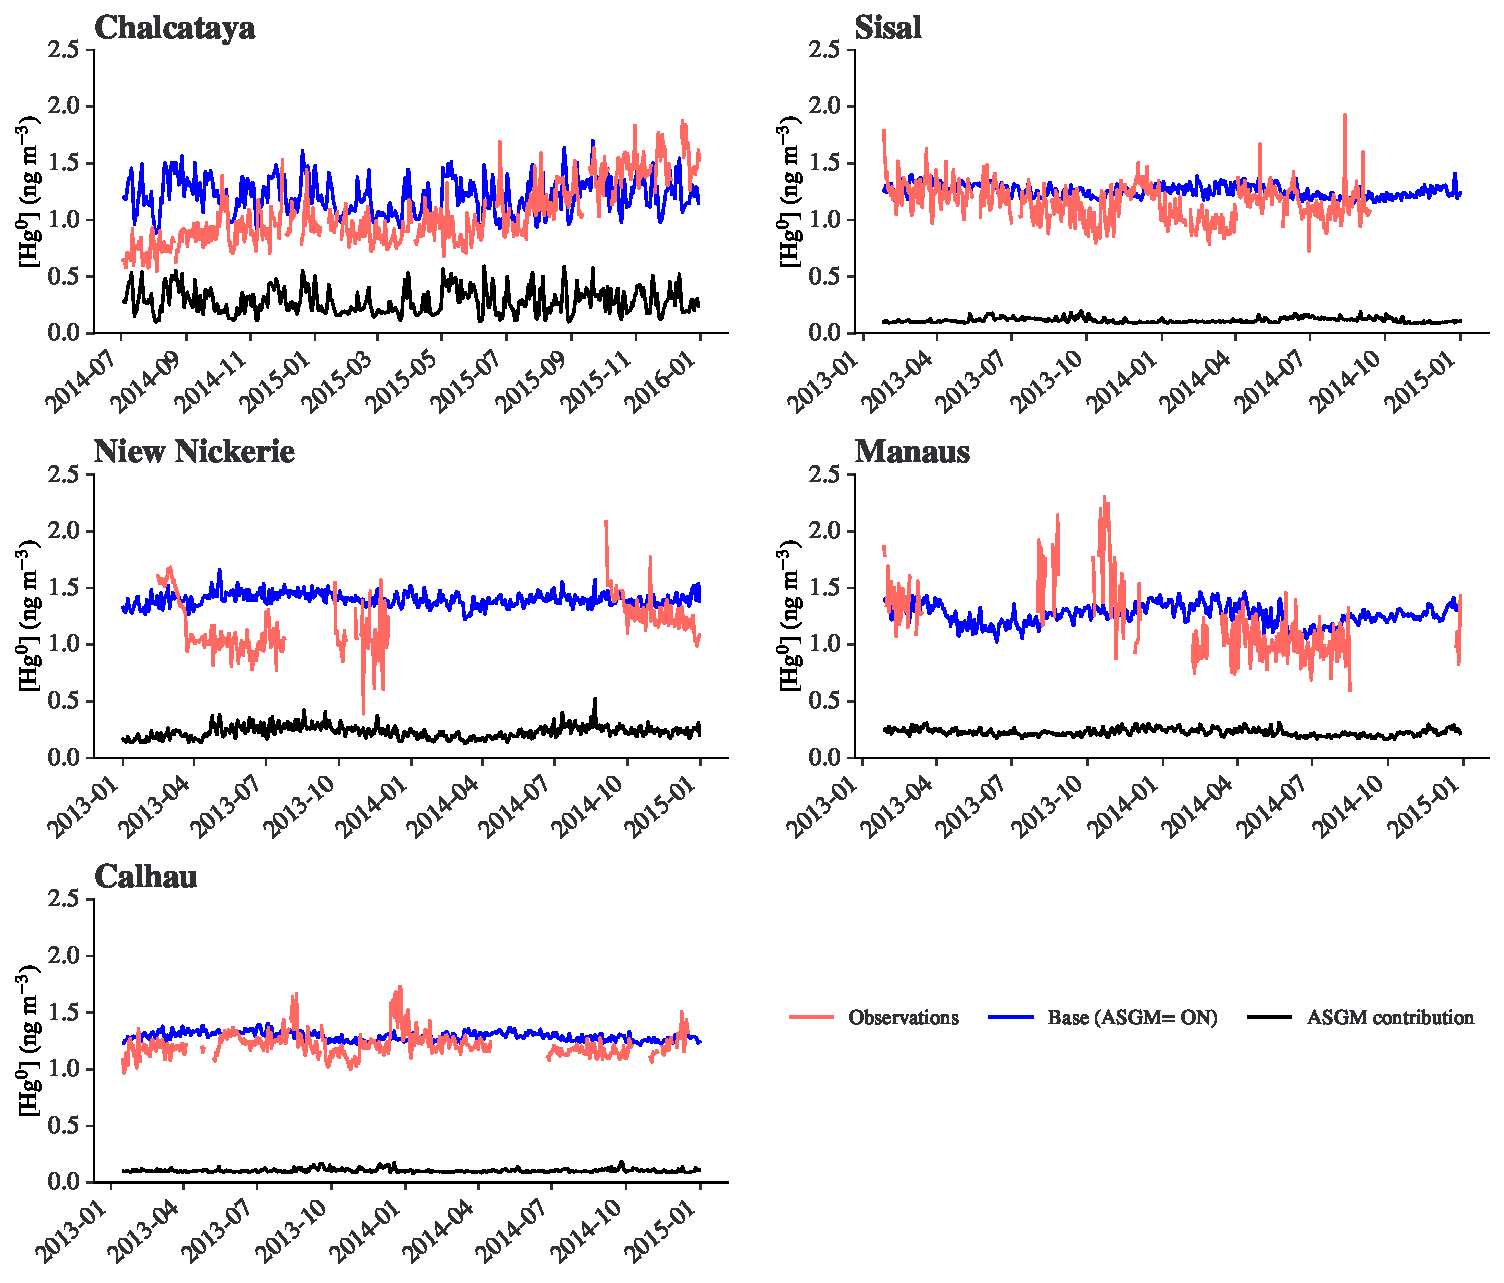
\includegraphics[width=\textwidth]{templates/figures/GMOS_Sites/GMOS_Sites.pdf}
\centering
\captionof{figure}{Time series plots of the observed TGM concentrations at different GMOS sites in red with the corresponding modeled concentration in blue and the associated ASGM contribution in black. Available observations and corresponding model output between January 2013 and January 2015 were plotted with the exception of the CHC site whose data is from July 2014 and January 2016}
\label{fig:GMOSvsGC}
\end{figure}
\FloatBarrier

\begin{flushleft}
Moreover, the Niew Nickerie and Manaus sites had the worst mean and variability relationship with the modelled \hg as seen on Table \ref{tab:modelvsobs metrics}. Even though the GEOS-Chem model overestimates the mean concentration over a one year period of measurement with the exception of the Manaus site as seen in Table \ref{tab:ASGM_at_GMOS_annual_avs}, the estimates for the mean concentration at Sisal and Calhau are within a 10\% margin as shown in Table \ref{tab:modelvsobs metrics}. The model's deficiency in predicting the mean may be the result of poor parameterization of processes such as dry deposition and wet deposition in the model. Poor parameterizations of ASGM Hg emissions in the model may also  contribute to the poor model skill in predicting the mean. Furthermore, the time series plot of the Hg concentrations at CHC show a general upward trend that is not represented in the other observations as well as the model. 
\end{flushleft}


\begin{flushleft}
  
\end{flushleft}

\begin{table}[H]
\captionof{table}{Table showing the extent to which the model predicts the observations showed by the percentage difference between the model predictions and the observations }
\label{tab:modelvsobs metrics}

\centering
\resizebox{0.5\textwidth}{!}{\begin{tabular}{lcc}
  \hline

GMOS  &Percentage difference & Percentage difference  \\
Site & annual mean (\%) & standard deviation (\%)           \\
                        
\hline
Sisal          & 6.72 &-64.29  \\
Calhau         & 6.56 &-66.66   \\
Niew Nickerie  & 27.03 &-73.91    \\
Manaus        & -14.77 &-70.97    \\
Chalcataya     &33.33 &-12.5   \\
  \hline
\end{tabular}}

\end{table}
\begin{flushleft}
 
\end{flushleft}


\subsection{Passive Sampler Observations vs GEOS-Chem}
\begin{flushleft}
 The comparison between the modelled concentration in the atmosphere and the PAS data corroborated the finding that the GEOS-Chem model overestimated the observed concentrations in the atmosphere as seen on Figure \ref{fig:06-12-22_pas_vs_model_Hg0-per-year_by-latitude_001} which shows the modeled (blue circles) and observed (red circles) annual average \hg plotted as a function of latitude. The observation error bars are represent the replicate precision of the observations while the model error bars represent the 95\textsuperscript{th} bootstrap confidence interval for the mean anual \hg. Moreover the PAS observations show high variability as you move from South to North while the model has low variability and and increasing trend.  
\end{flushleft}

\begin{figure}[H]
  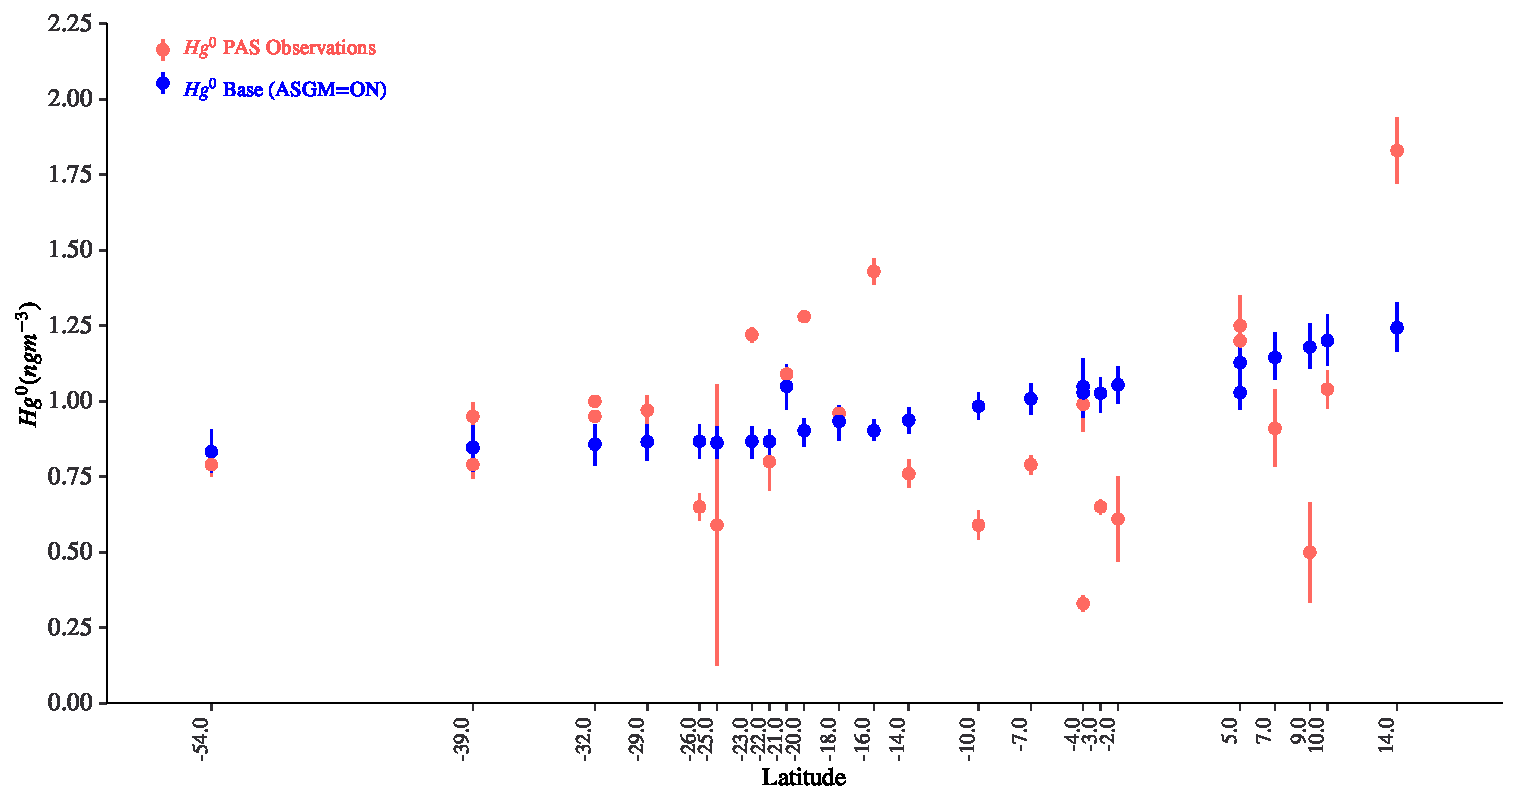
\includegraphics[width=\textwidth]{templates/figures/Passive_Samplers/06-12-22_pas_vs_model_Hg0-per-year_by-latitude_001.pdf}
  \caption{\hg in the atmosphere as a function of Latitude. The \on (blue circles) and observed (red circles) annual average \hg plotted are plotted as a function of latitude to evaluate spatial trends across the continent. The observation error bars are represent the replicate precision of the observations while the model error bars represent the 95\textsuperscript{th} bootstrap confidence interval for the mean annual \hg.}
  \label{fig:06-12-22_pas_vs_model_Hg0-per-year_by-latitude_001}
  \centering
  
\end{figure}
\FloatBarrier

\begin{flushleft}
GEOS-Chem's poor predictive capacity observed above is also addressed in Feinberg et al. (2022) where we evaluated atmospheric Hg uptake by vegetation in \gc by constraining vegetation as an Hg sink through comparison of simulations with a compiled database of litterfall, throughfall and flux tower tower measurements from 93 forested sites. We found that the \gc version, 12.8  underestimated dry deposition of \hg which may explain why the observed Hg from the measurements of Hg in the atmosphere at different sites in Latin America was lower than the concentration predicted by the model. Recent studies evaluating the global biogeochemical cycle of Hg argue that Hg concentrations in the atmosphere exhibit an inter-hemispheric gradient from the southern to the northern hemisphere. The annual average \hg modelled by \gc seems to follow the proposed gradient as seen on Figure \ref{fig:06-12-22_pas_vs_model_Hg0-per-year_by-latitude_001}. Furthermore, the PAS measurements as seen on Figure \ref{fig:06-12-22_pas_vs_model_Hg0-per-year_001} were higher in most of the eastern coastal regions and in the north western coastal regions. These high values are the result of the fact that the PASs were placed in close proximity to populated area where the Hg background in the atmosphere may also be influenced by Hg emission sources such as power generation and ASGM.

\end{flushleft}

\begin{figure}[H]
  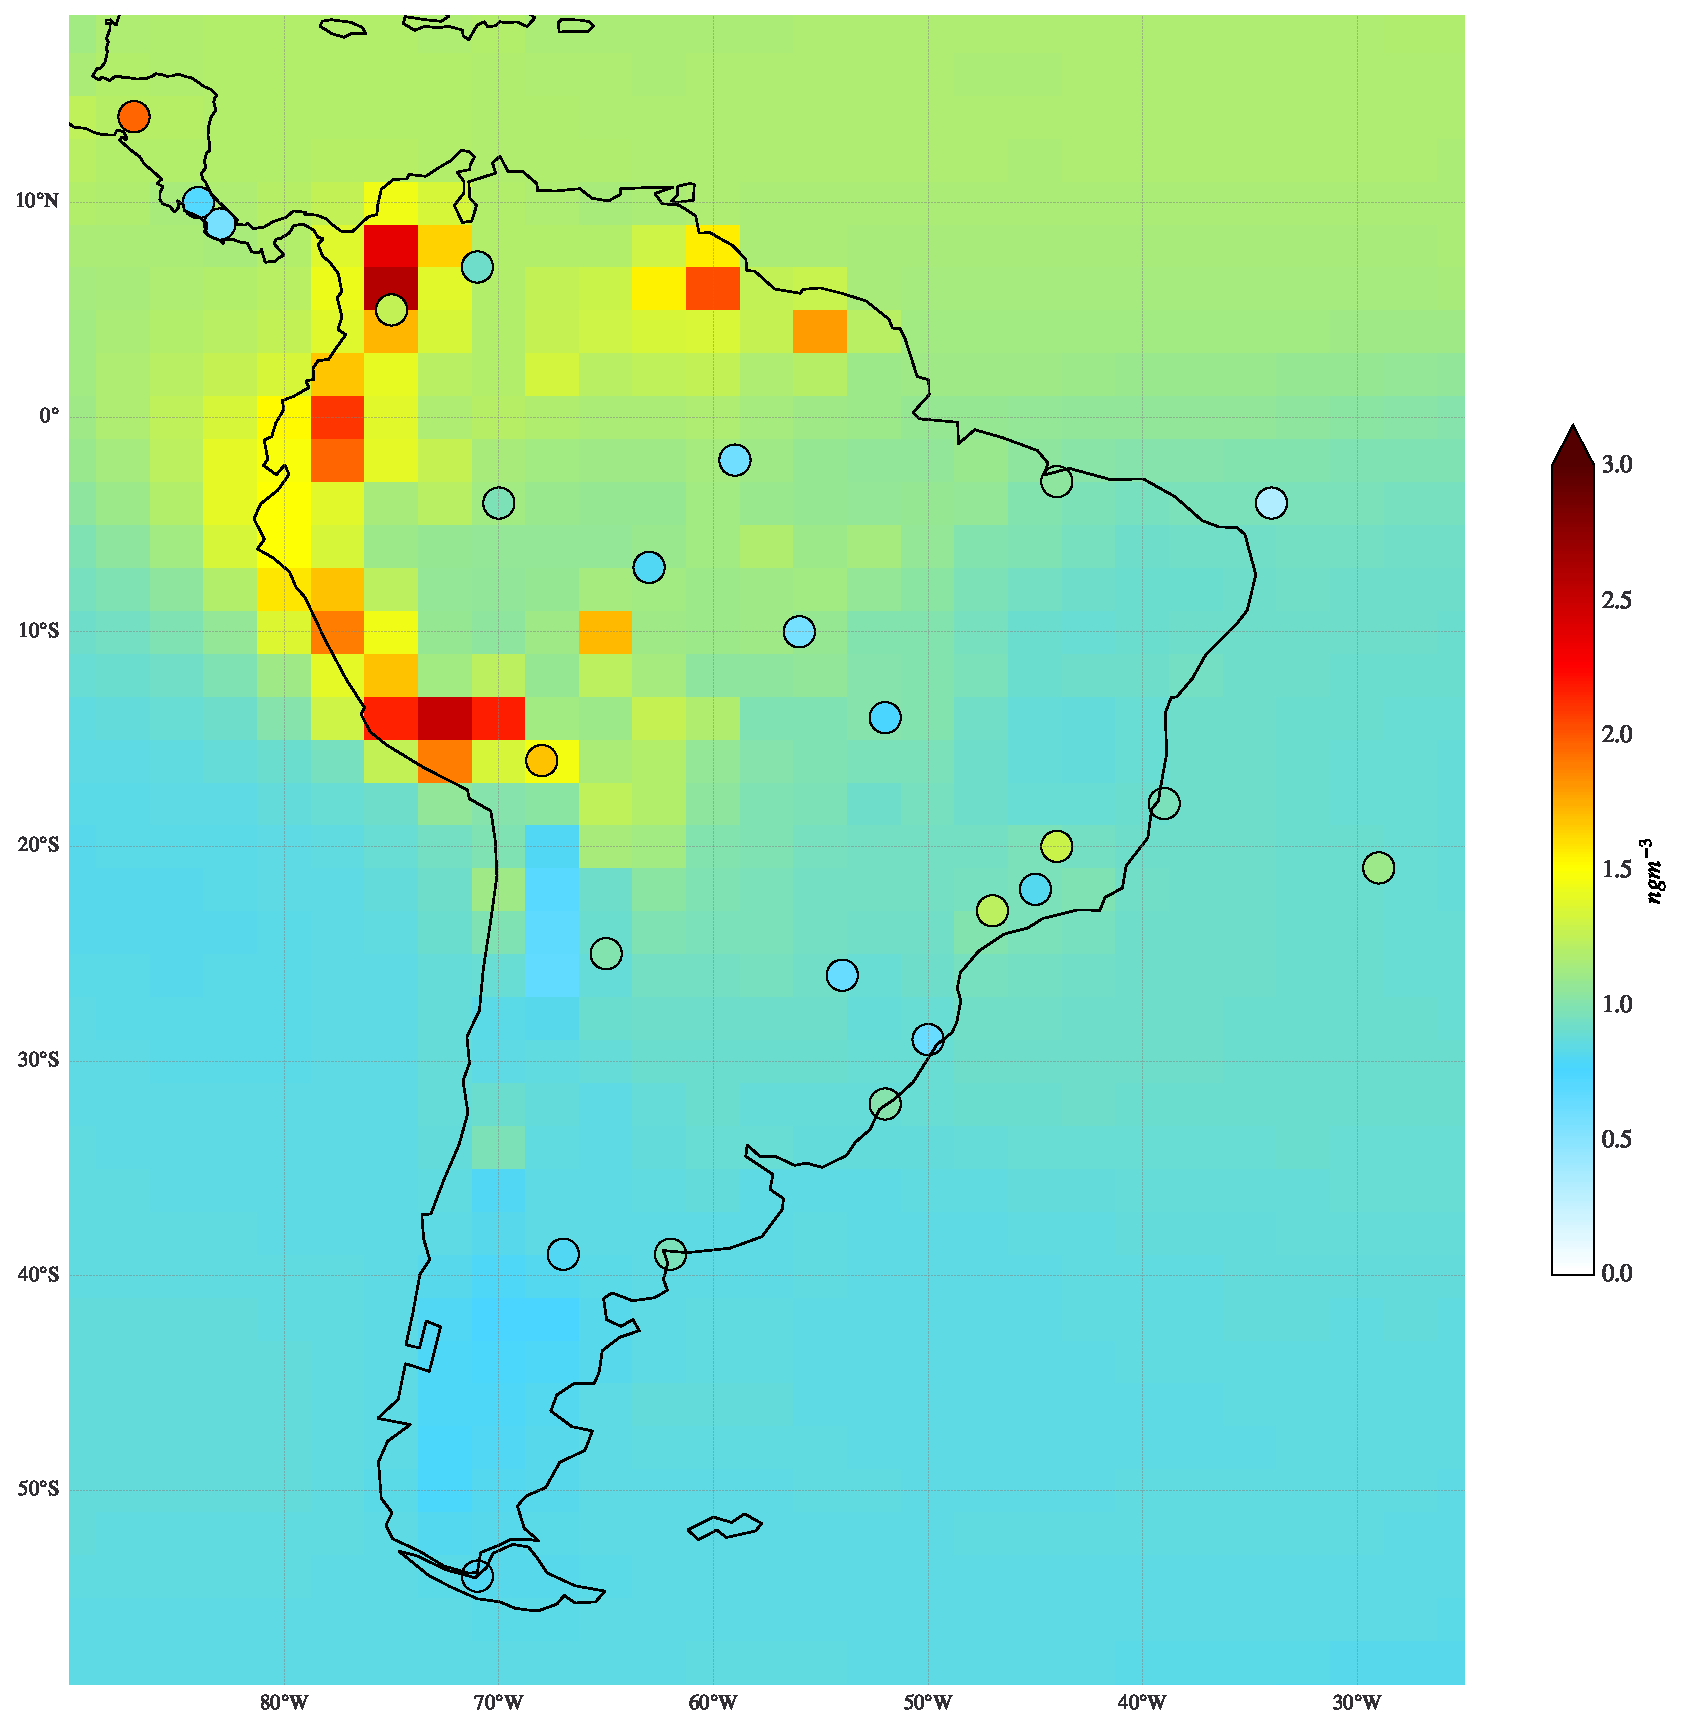
\includegraphics[width=0.7\textwidth]{templates/figures/Passive_Samplers/06-12-22_pas_vs_model_Hg0-per-year_001.pdf}
  \caption{Surface \hg over Latin America averaged over the course of one year, 2015.The figure compares the the annual average \hg produced by the \on (background grid) with the PAS measurements (circles).}
  \label{fig:06-12-22_pas_vs_model_Hg0-per-year_001}
  \centering
  
\end{figure}
\FloatBarrier



\subsection{Observed Hg Concentration at CHC}
\begin{flushleft}
The time series of the observed concentration at the CHC station between July 2014 and January 2016 is shown on Figure\ref{fig:ObsTseries}. The detailed characteristics of the observations over this measurement period were described in Koening et al.,(2020); hence our analysis was focused on using the observation TGM data to evaluate the performance of the GEOS-Chem model in predicting the \hg based on the input \hg emission inventories. As shown by the plot of the \hg 120 day moving as a function of time on Figure\ref{fig:ObsTseries}, we found that the observed TGM concentration in the atmosphere had a visible upward trend, which Koening et al.,(2020) attribute to the El Niño-Southern Oscillation (ENSO). Consequently, Koening et al.,(2020) categorized the measured TGM concentrations in the atmosphere at the CHC site into normal conditions (NC), 2014-07 to 2015-05 and ENSO conditions  2015-06 to 2016-01. The meteorology associated with ENSO was not accounted for in the GEOS-Chem \hg simulations we conducted; therefore the simulated \hg  at CHC was compared to the TGM observations for the one year period between 2014-07-02 to 2015-07-02.
\end{flushleft}

\begin{figure}[H]
  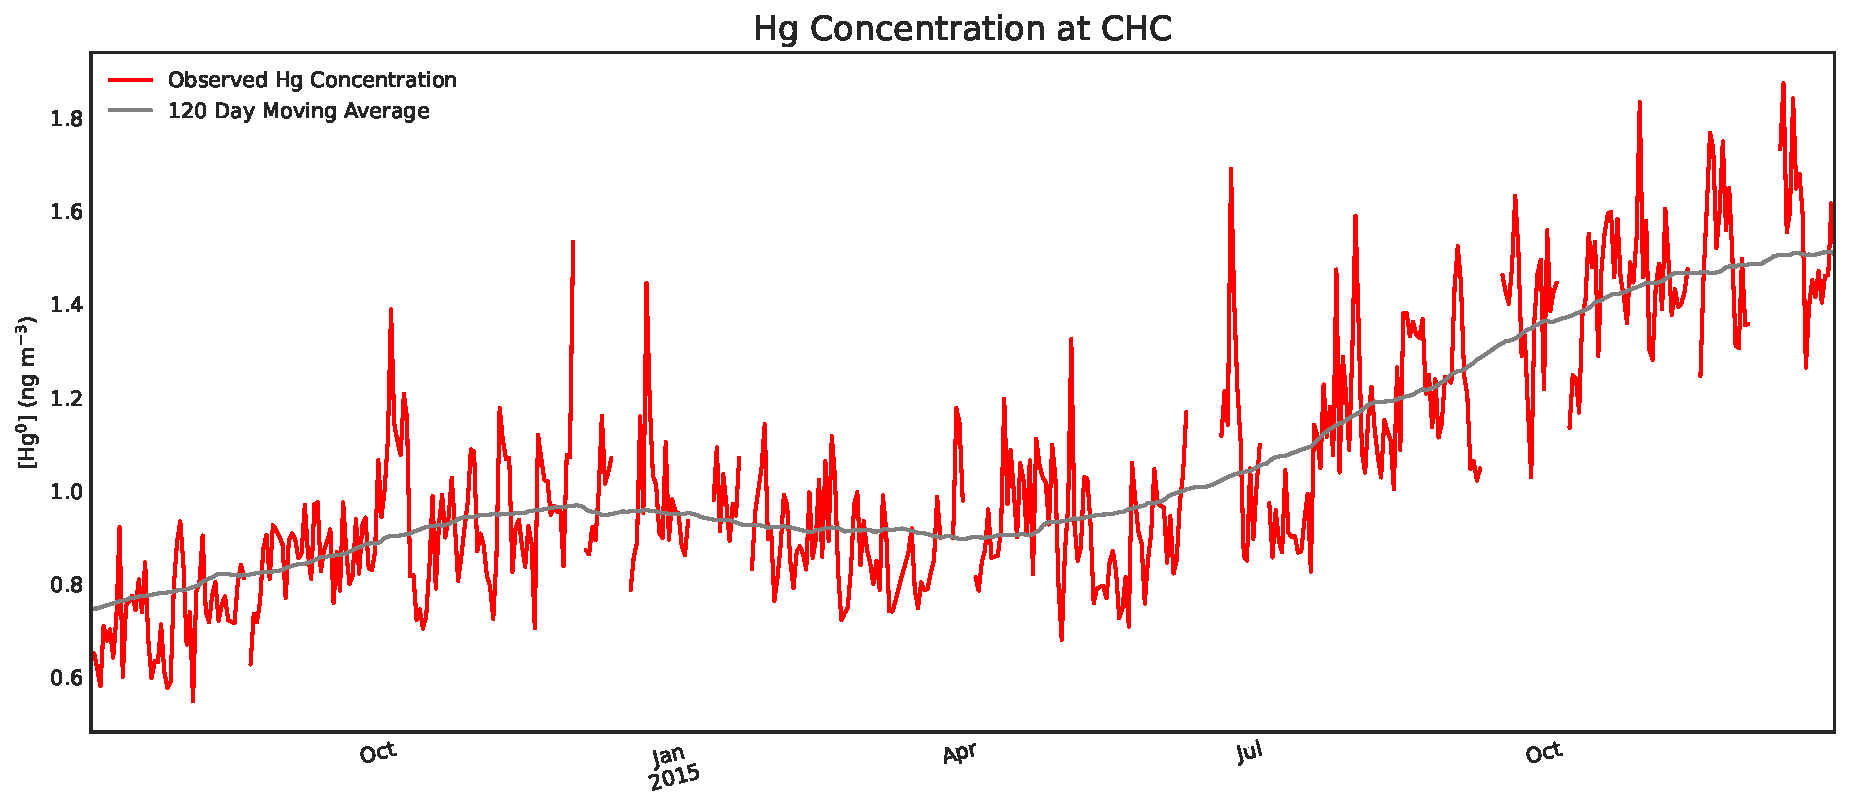
\includegraphics[width=\textwidth]{templates/figures/GMOS_Sites/ObsTimeSeries.pdf}
 
  \caption{The average daily TGM concentration at CHC in ngm\textsuperscript{-3} as a function of time over the measurement period from July 2014 to January 2016. The daily average concentration in indicated by the red line while the grey line shows the 120 day moving average which clearly highlights the upward trend in the daily averages}
  \label{fig:ObsTseries}
  \centering
\end{figure}
\FloatBarrier

\begin{flushleft}
  Figure \ref{fig:ModelvsObsNstats} the detailed comparison between the simulated \hg  and the observed TGM concentration at CHC. The observations (in red) are plotted as a function of time in (a) with the Base (ASGM= OFF) simulation (in green) and (c) with the Base (ASGM= ON) simulation in (blue). The scatter plots in (b) and (d) represent the modeled \hg  as a function of the measured TGM concentration. The scatter plot in plot (b) the variability in the observed TGM concentration is not captured by the Base (ASGM= OFF) simulation while the scatter plot in (d) shows that the Base (ASGM=ON) simulation over estimates the observed values even though it matches the variability in the values. The dispersion around the 1:1 line is substantial in both scatter plots and hence the correlation coefficient is low in both cases. 
\end{flushleft}


\begin{figure}[H]
  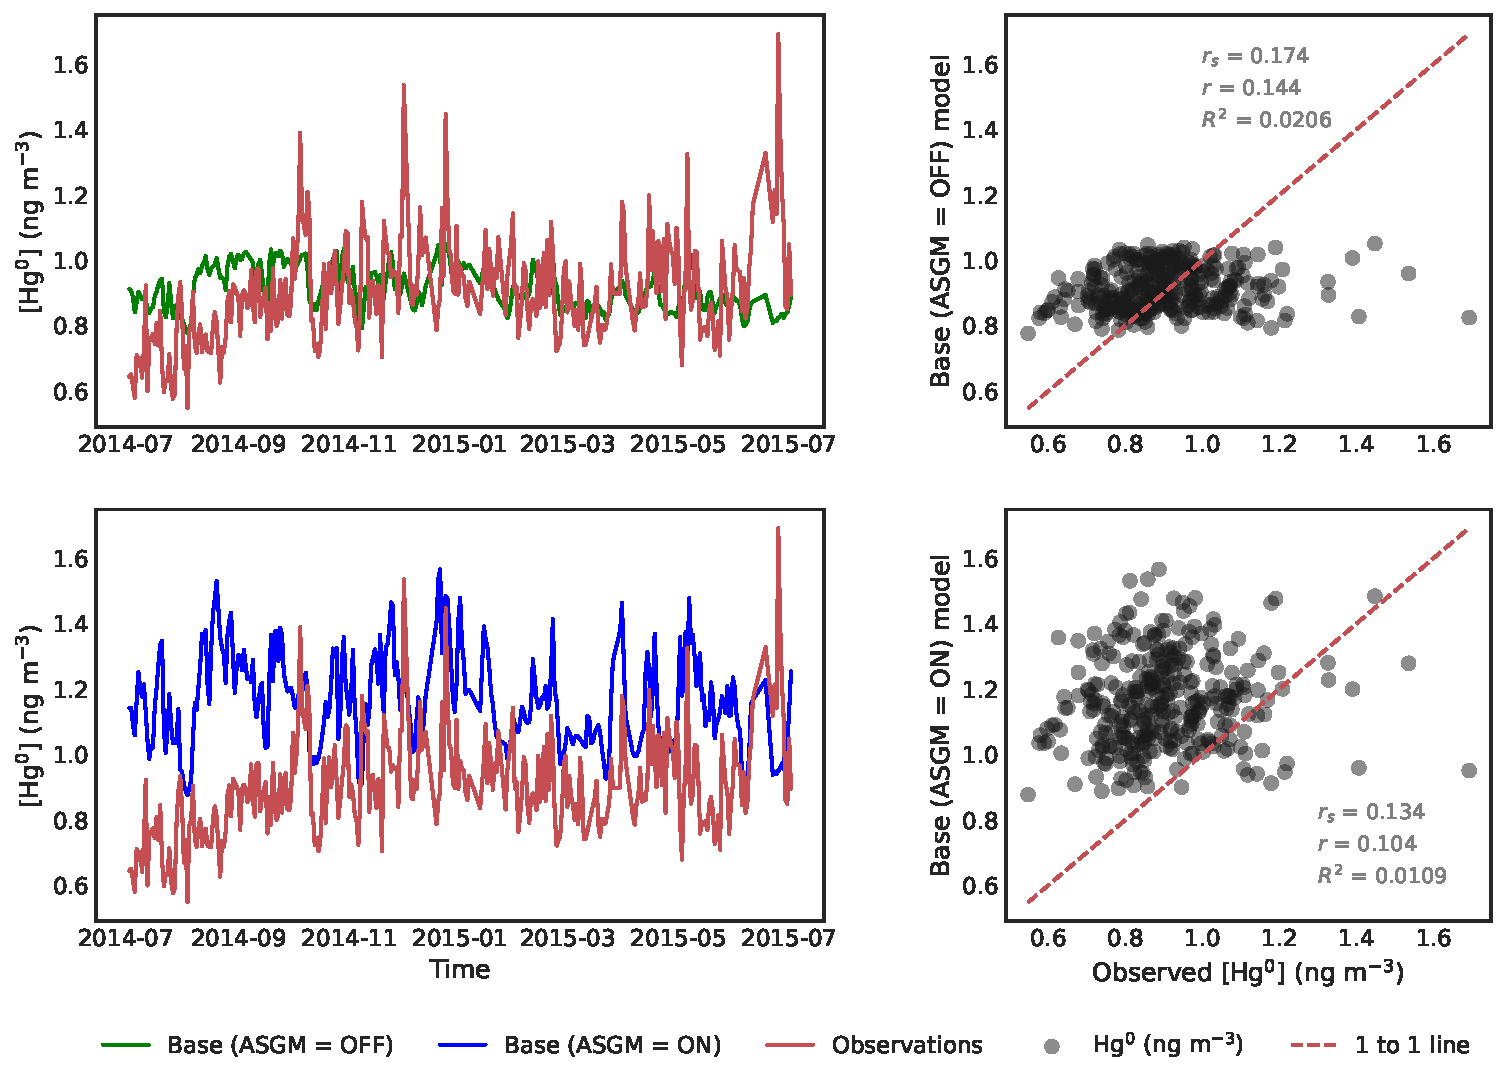
\includegraphics[width=\textwidth]{templates/figures/ModelvsObs/TimeSeriesNsactter_obsVmodel_v1.pdf}
  \centering
  \caption{Observed vs modelled (3 different simulations) Hg concentration at CHC and scatter plots of how the model compares with the observations  }
  \label{fig:ModelvsObsNstats}
\end{figure}
\FloatBarrier
\begin{flushleft}
We also found that the mean \hg concentration produced by the Base (ASGM= OFF) simulation was within 1\% of the observed TGM concentration as seen on Table \ref{tab:ModelvsObsStats} where $\mu$ is the annual average Hg concentration, $\sigma$ is the standard deviation, $iqr$ is the interquartile range, $r_s$ is the Spearman correlation, $r$ is the Pearson correlation, and $R^2$ is the coefficient of determination. On the contrary, the average \hg produced by the \on shown by the blue line plot on Figure \ref{fig:ModelvsObsNstats} overestimated the mean by 29\%.
 
\end{flushleft}
\setlength{\tabcolsep}{2.5pt}
\begin{table}[H]
  \begin{center}
    \caption{Characteristics of observed and modelled Hg concentration in CHC where$\mu$ is the annual average Hg concentration, $\sigma$ is the standard deviation, $iqr$ is the interquartile range, $r_s$ is the Spearman correlation, $r$ is the Pearson correlation and $R^2$ is the coeeficient of determination}
    \label{tab:ModelvsObsStats}
    \begin{tabular}{lcccccc}
       %<-- added & and content for each column
      
                          & $\mu$                 & $\sigma$            & $iqr$               & & & \\
                          &  (ng m$^{-3}$)/year)  & (ng m$^{-3}$)/year) & (ng m$^{-3}$)/year) & & & \\
     \cmidrule{2-4}
     Observations         & 0.90             & 0.16            & 0.18        &  & & \\
     \textbf{Simulations} &                  &                  &               &\textbf{$r_s$} &\textbf{$r$} &\textbf{$R^2$}\\ %
      \hline
      Base (ASGM=OFF)     & 0.91             & 0.06            & 0.11         & 0.17         & 0.144      & 0.0196\\ 
      Base (ASGM=ON)      & 1.16            & 0.14            & 0.20        & 0.124         & 0.101       & 0.0102\\ % <--
    \end{tabular}
  \end{center}
\end{table}
\FloatBarrier

\begin{flushleft}
Even though GEOS-Chem reproduced the mean Hg concentrations at CHC in the \off, the Spearman ($r_s$) and Pearson ($r$) correlations between the modelled and observed concentrations were very low at 1.63e-1 and 1.40e-1 respectively. Moreover, the coefficient of determination, $R^2$ between the observed and modelled concentrations in \on case was almost zero at 0.021. Also, the \on did not reproduce the variability in the observed concentrations as evident in Figure \ref{fig:ModelvsObsNstats} and in Table \ref{tab:ModelvsObsStats} where we gleaned that the observations had more than twice the modelled variance in the \on case. Brasseur and Jacob,(p.471 2017) assert that in cases where a model captures the observed means but not the observed variability, the mean may be wrongly interpreted \cite{brasseur_modeling_2017}. In the case of \off, the mean may be wrongly interpreted because of the exclusion of the ASGM Hg emissions. In addition, we found that turning on ASGM emissions in GEOS-Chem led to  atmospheric Hg concentrations that had a variance comparable with the observed variance. However, we also discovered that turning on ASGM emissions in the model did not lead to improvements in the correlation between the modeled and observed \hg in the atmosphere. 
The relationship between the mean and variance in the observed and modeled  atmospheric Hg concentration at CHC was further explored as shown on Figure \ref{fig:Histplots} which shows the extent to which the GEOS-Chem model reproduces the mean and IQR of the observations. Even though the \on  better recreated the IQR of the Hg concentration in the atmosphere, the mean \hg in this simulation was almost two standard deviations away from the mean of the observations. The above comparison indicates that the mean was not a good metric to investigate the relationship between the Hg concentration in the atmosphere and ASGM emissions as modelled by GEOS-Chem. 
\end{flushleft}



\begin{figure}[H]

\begin{tabular}[H]{cc}

\subfloat[]{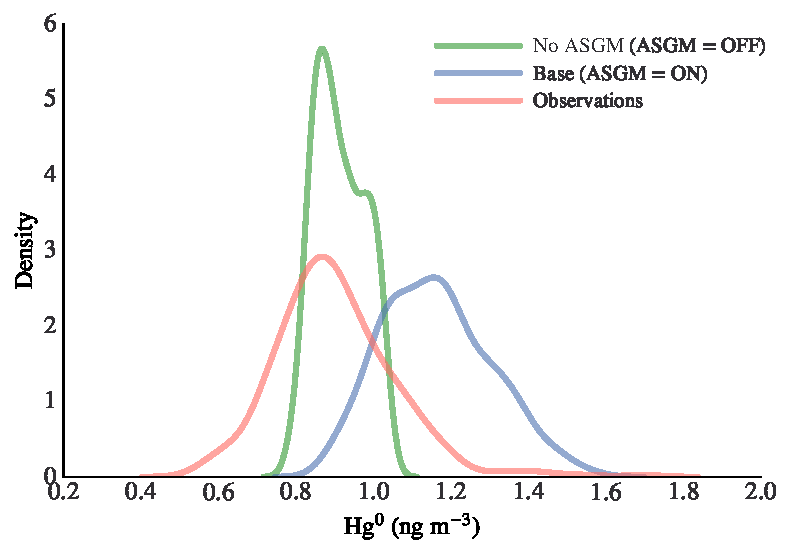
\includegraphics[width = 0.5\linewidth]{templates/figures/ModelvsObs/06-12-22_models_vs_observations_density-plot.pdf}} &
\subfloat[]{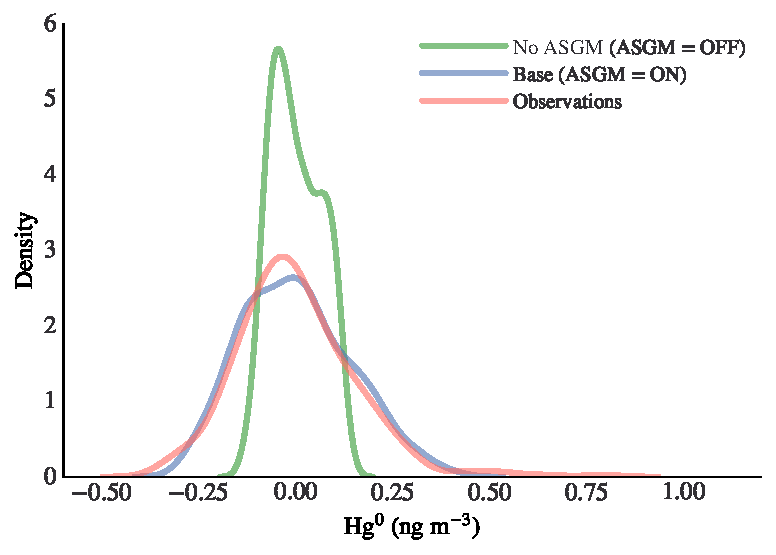
\includegraphics[width = 0.5\linewidth]{templates/figures/ModelvsObs/06-12-22_models_vs_observations_density-plot_std.pdf}}
\end{tabular}
\centering
\captionof{figure}{Plots Showing Data and Modeling  Results from GMOS Monitoring Network Sites in South America}
\label{fig:Histplots}
\end{figure}
\FloatBarrier

\begin{flushleft}
Instead, the IQR and 95$^{th}$ percentile range were found to be metrics that were informative about the effect of ASGM on the simulated Hg concentration site at distant high altitude measuring station site. The failure of GEOS-Chem to reproduce the observed mean Hg concentration at a high altitude measuring site may be attributed to poor parameterizations in the model such as the influence of dry deposition. The flaws in the GEOS-Chem Hg dry deposition scheme in version 12.8.1 of GEOS-Chem used in this analysis were discussed in detail and improved in Feinberg et.al (2022). Furthermore, we hypothesized that poor spatial distribution of emissions in the 2015 Hg ASGM emissions inventory which are an input to the GEOS-Chem may have also contributed to the model observation mismatches. 

\end{flushleft}






\section{Conclusion}

